\documentclass[border=3mm]{standalone}
\usepackage{tikz}

\newcommand{\SierpinskiCarpet}[4]{%
  \ifnum#4>0\relax
    \pgfmathsetmacro{\s}{#3/3}

    \pgfmathsetmacro{\cx}{#1+\s}
    \pgfmathsetmacro{\cy}{#2+\s}

    \fill[white] (\cx,\cy) rectangle ++(\s,\s);

    \edef\nextdepth{\number\numexpr#4-1\relax}

    \foreach \i in {0,1,2}{
      \foreach \j in {0,1,2}{
        \ifnum\i=1\relax
          \ifnum\j=1\relax
          \else
            \pgfmathsetmacro{\nx}{#1+\i*\s}
            \pgfmathsetmacro{\ny}{#2+\j*\s}
            \SierpinskiCarpet{\nx}{\ny}{\s}{\nextdepth}
          \fi
        \else
          \pgfmathsetmacro{\nx}{#1+\i*\s}
          \pgfmathsetmacro{\ny}{#2+\j*\s}
          \SierpinskiCarpet{\nx}{\ny}{\s}{\nextdepth}
        \fi
      }
    }
  \fi
}

\begin{document}
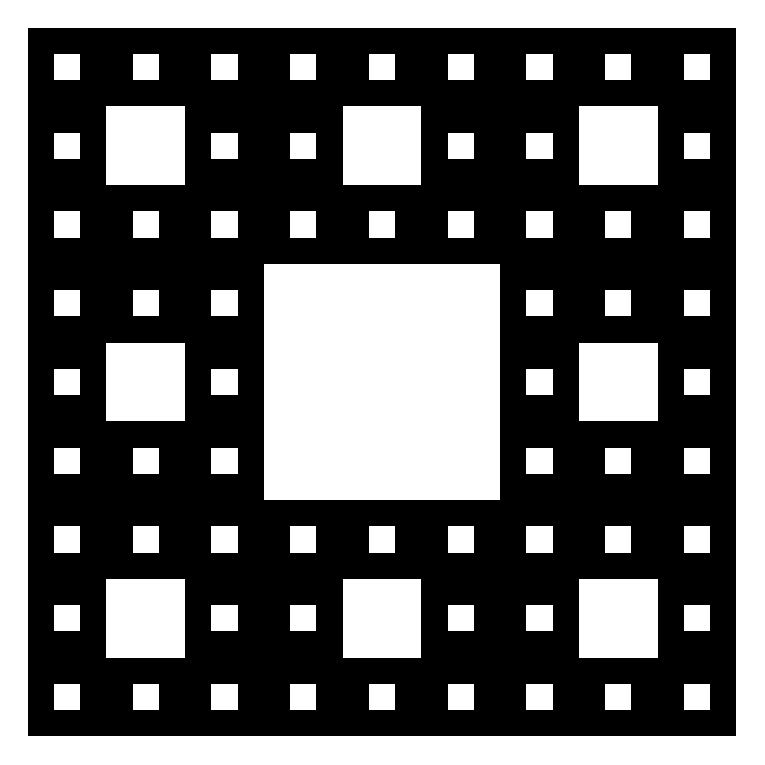
\begin{tikzpicture}

\def\Size{9} 
\def\Depth{3} 

\fill[black] (0,0) rectangle (\Size,\Size);

\SierpinskiCarpet{0}{0}{\Size}{\Depth}

\end{tikzpicture}
\end{document}
